\documentclass[10pt]{exam}
\usepackage[hon]{template-for-exam}
\usepackage{silence,tikz,multicol}
\WarningFilter{latex}{Label `question}
\WarningFilter{latex}{There were multiply-defined labels}
\usepackage{pgfplots}
\pgfplotsset{
    compat=1.18,
    pulseplot/.append style={
      xmin =-6.5,
      xmax = 6.5,
      ymin =-2.5,
      ymax = 2.5,
      axis lines = none,
      xtick = {},
      ytick = {},
      height = 5cm,
      width = 7.5cm,
      grid = major,
      grid style = {thick, dotted},
      tick label style = {font=\small}
    },
  }
\pgfmathdeclarefunction{gauss}{2}{%
  \pgfmathparse{1/(#2*sqrt(2*pi))*exp(-((x-#1)^2)/(2*#2^2))}%
}

\title{Sound \& Waves Stations}
\author{Rohrbach}
\date{\today}

\begin{document}
\maketitle

\section{Section 20.1 : The Nature of Sound}

Read Section 20.1 (pp. 375-376)

\begin{questions}
  \question 
    How are sound waves produced? \vs

  \question 
    What type of wave is a sound wave? \vs

  \question 
    Define the following terms:

    \begin{parts}
      \part pitch \vspace{2em}
      \part infrasonic \vspace{2em}
      \part ultrasonic \vspace{2em}
    \end{parts}

  \question 
    What sorts of materials cause sound to travel more quickly?  Why? \vs

\end{questions}

\section{Function Generator and Speaker}

\begin{questions}
  \question
    Adjust the frequency and the amplitude.  Describe what you notice about the sound. \vs

  \question
    Start the frequency very low (2 Hz or smaller).  Slowly increase the frequency until it starts to sound like a tone.  This is the point at which the sound stops being \emph{infrasonic}.  Write down this frequency. \vs


  \question
    Start the frequency very high (Above 40,000 Hz).  Slowly decrease the frequency until you can hear it.  This is the point at which the sound stops being \emph{ultrasonic}.  Write down this frequency.  When you are finished, {\bf please make sure to turn the amplitude all the way down so it doesn't bother your classmates}. \vs

\end{questions}

\pagebreak


\section{Acoustic Beats}

  You will define the term ``acoustic beats'' in a moment.  But, in the meantime, let's experience what beats are.  There are two tuning forks in front of you.  One has adjustable weights.  Make sure each of the weights is lined up with the indented line on the tuning fork.  Hit each tuning fork.  They should sound the same.

  \begin{questions}
  
    \question 
      After having heard the two tuning forks playing the same frequency, change the frequency of the adjustable tuning fork slightly by lowering one of the weights by 1-2 centimeters.  Play both tuning forks again.  Explain what you are hearing.  \vs

    \question
      This ``throbbing'' or ``wobbling'' you are hearing is called ``acoustic beats.'' Read Section 20.8 (pp. 385-386). What are ``\emph{beats}''? \vs
    \question
      In experiencing beats, why does the sound switch from loud to soft to loud to soft? \vs
    \question
      Move the weight even further and play the tuning forks.  You should notice that the ``throbbing'' changes frequency.  Does it shift to a higher frequency or a lower frequency? \vs
    \question
      To explain why beats occur, take a look at the two pendulums hanging at your station.  They are different lengths, which means they have different periods and different frequencies.  Set them both in motion and watch what happens.  Do they ever look like they are in sync?  Do they ever look like they're out of sync? \vs


  \question
    Look at the diagram below (Figure 20.21 from the textbook).  Label the regions of constructive and destructive interference.

    \begin{tikzpicture}
      \node at (0,0) 
        {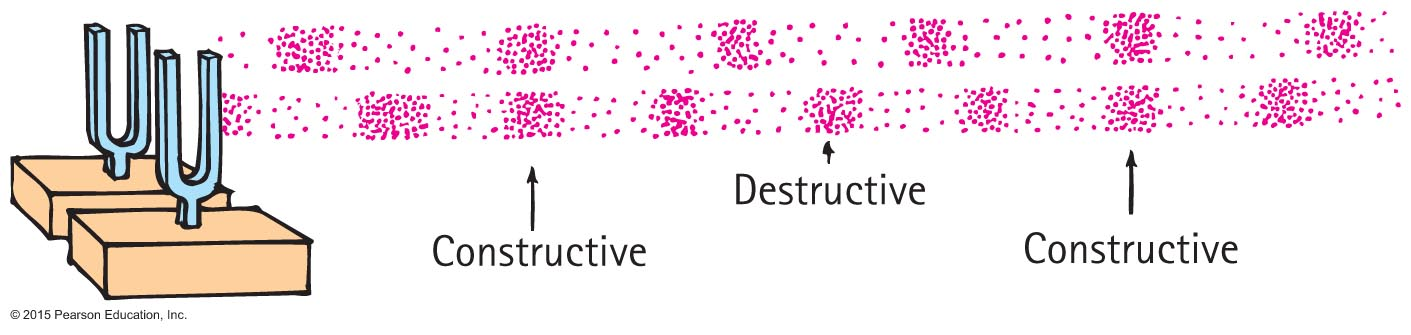
\includegraphics[width=12cm]{Fig20_21.jpg}};
      \fill[white] (-3,-1) rectangle (6,.26);
    \end{tikzpicture}
 
  % \question
  %   Draw your own beats!  Draw two bunnies hopping forward.  One bunny jumps forward 3 cm each hop; the other bunny jumps forward 4 cm each hop.  Circle the locations where the bunnies are `'`in sync.''

  %   \begin{tikzpicture}
  %     \draw[dotted] (0,0) grid[step=0.5] (15,-1.5);
  %     \fill (0,-0.5) circle (0.1)
  %       ++ (1.5,0) circle (0.1)
  %       ++ (1.5,0) circle (0.1);
  %     \fill (0,-1) circle (0.1)
  %       ++ (2,0) circle (0.1)
  %       ++ (2,0) circle (0.1);
  %   \end{tikzpicture}
\end{questions}

\pagebreak

\section{Resonance Tube}

\begin{questions}
  \question \label{def-resonance}
    Take a look at the resonance page of your notes.  What is \emph{resonance}? \vs

  \question
    Hit the tuning fork against the table to generate a tone.  Hold it over the resonance tube.  Keep changing the length of the resonance tube until you hear the sound get louder.  What is happening and why? \vs

  \question
    Looking at your answer to \#\ref{def-resonance}, what do you think you are changing when you change the length of the tube? \vs

  \question
    Now, turn on the function generator.  Gradually change the frequency.  Pay attention to what happens to each of the three metal sheets.  Explain why you think that they don't all resonate at the same time. \vs
    
\end{questions}


\section{Slinkies}

\begin{questions}

  \question
    Send a {\bf transverse} pulse (one at a time, and just one person) down a stretched slinky.  Send a large pulse and a small pulse down the slinky. Which one appears to travel faster? 
    \vs
  
  \question
    Send a large pulse and a small pulse down the slinky. Which one appears to travel faster? 
    \vs
  
  \question
    Change the tension of the spring by coming closer together or moving further apart.  How (if at all) does tension in the slinky seem to affect the speed of the wave?
    \vs
  
  \question
    Send another transverse pulse.  What happens to the orientation of the wave (right side up or upside down) when it reaches the other side of the slinky and bounces back?
    \vs

      

  \pagebreak
  
  \question
    Stretch the large spring and send a {\bf longitudinal} pulse down the spring.  Observe the motion of the spring coils.  How are they moving?
    \vs

  \question
    Have each person send a {\bf singular wave pulse} down the spring at the same time.  Make sure the amplitudes of the waves are on the {\bf same} side of the spring.  
  
    \begin{parts}
      \part 
        Do the waves bounce off each other or pass through each other?

        \begin{flushright}
          \begin{tikzpicture}
            \begin{axis}[pulseplot]
              \addplot[smooth,domain=-6:6,samples=50,ultra thick] {1.3*(gauss(-4,.5)+gauss(4,.5))};
              \draw[->,thick] (-3,.7) -- (-2,.7);
              \draw[->,thick] (3,.7) -- (2,.7);
            \end{axis}
          \end{tikzpicture}
        \end{flushright}


      \part 
        What do you observe where the waves meet (in the middle)? \vs
      \part 
        Which kind of interference is this? \vs 
    \end{parts}
  
  
  \question
    Have each person send a singular wave pulse down the spring at the same time.  Make sure the amplitudes of the waves are on the {\bf opposite} sides of the spring.  What do you notice?
  
    \begin{parts}
      \part 
        Do you think the waves bounce off each other or pass right through?

        \begin{flushright}
          \begin{tikzpicture}
            \begin{axis}[pulseplot]
              \addplot[smooth,domain=-6:6,samples=50,ultra thick] {1.3*(gauss(-4,.5)-gauss(4,.5))};
              \draw[->,thick] (-3,.7) -- (-2,.7);
              \draw[->,thick] (3,-.7) -- (2,-.7);
            \end{axis}
          \end{tikzpicture}
        \end{flushright}

      \part 
        What do you observe where the waves meet (in the middle)? \vs
      \part 
        Which kind of interference is this? \vs 
    \end{parts}

    
  \question
    While holding one end of the large spring firmly in place, move the other end of the spring continuously back and forth to send a continuous wave down the spring. See if you can achieve the third, fourth, and fifth harmonics.  Draw your results
  
    \begin{tikzpicture}
      \draw[dotted] (0,0) grid[step=0.5cm] (15,5);
    \end{tikzpicture}
  
  

\end{questions}


\end{document}